\def\year{2020}\relax
%File: formatting-instruction.tex
\documentclass[letterpaper]{article}% DO NOT CHANGE THIS
\usepackage{aaai20}  				% DO NOT CHANGE THIS
\usepackage{times}  				% DO NOT CHANGE THIS
\usepackage{helvet} 				% DO NOT CHANGE THIS
\usepackage{courier}  				% DO NOT CHANGE THIS
\usepackage[hyphens]{url}  			% DO NOT CHANGE THIS
\usepackage{graphicx} 				% DO NOT CHANGE THIS
\usepackage[backend=bibtex, style=numeric]{biblatex}
\urlstyle{rm} 						% DO NOT CHANGE THIS
\def\UrlFont{\rm}  					% DO NOT CHANGE THIS
\usepackage{graphicx}  				% DO NOT CHANGE THIS
\frenchspacing  					% DO NOT CHANGE THIS
\setlength{\pdfpagewidth}{8.5in}  	% DO NOT CHANGE THIS
\setlength{\pdfpageheight}{11in}  	% DO NOT CHANGE THIS
%\nocopyright
%PDF Info Is REQUIRED.
% For /Author, add all authors within the parentheses, separated by commas. No accents or commands.
% For /Title, add Title in Mixed Case. No accents or commands. Retain the parentheses.
 \pdfinfo{
/Title (Predizioni attraverso GA e LSTM basate sul Covid-19)
/Author (Luca Perali, Michele Thiella)
} %Leave this	
% /Title ()
% Put your actual complete title (no codes, scripts, shortcuts, or LaTeX commands) within the parentheses in mixed case
% Leave the space between \Title and the beginning parenthesis alone
% /Author ()
% Put your actual complete list of authors (no codes, scripts, shortcuts, or LaTeX commands) within the parentheses in mixed case. 
% Each author should be only by a comma. If the name contains accents, remove them. If there are any LaTeX commands, 
% remove them. 

% DISALLOWED PACKAGES
% \usepackage{authblk} -- This package is specifically forbidden
% \usepackage{balance} -- This package is specifically forbidden
% \usepackage{caption} -- This package is specifically forbidden
% \usepackage{color (if used in text)
% \usepackage{CJK} -- This package is specifically forbidden
% \usepackage{float} -- This package is specifically forbidden
% \usepackage{flushend} -- This package is specifically forbidden
% \usepackage{fontenc} -- This package is specifically forbidden
% \usepackage{fullpage} -- This package is specifically forbidden
% \usepackage{geometry} -- This package is specifically forbidden
% \usepackage{grffile} -- This package is specifically forbidden
% \usepackage{hyperref} -- This package is specifically forbidden
% \usepackage{navigator} -- This package is specifically forbidden
% (or any other package that embeds links such as navigator or hyperref)
% \indentfirst} -- This package is specifically forbidden
% \layout} -- This package is specifically forbidden
% \multicol} -- This package is specifically forbidden
% \nameref} -- This package is specifically forbidden
% \natbib} -- This package is specifically forbidden -- use the following workaround:
% \usepackage{savetrees} -- This package is specifically forbidden
% \usepackage{setspace} -- This package is specifically forbidden
% \usepackage{stfloats} -- This package is specifically forbidden
% \usepackage{tabu} -- This package is specifically forbidden
% \usepackage{titlesec} -- This package is specifically forbidden
% \usepackage{tocbibind} -- This package is specifically forbidden
% \usepackage{ulem} -- This package is specifically forbidden
% \usepackage{wrapfig} -- This package is specifically forbidden
% DISALLOWED COMMANDS
% \nocopyright -- Your paper will not be published if you use this command
% \addtolength -- This command may not be used
% \balance -- This command may not be used
% \baselinestretch -- Your paper will not be published if you use this command
% \clearpage -- No page breaks of any kind may be used for the final version of your paper
% \columnsep -- This command may not be used
% \newpage -- No page breaks of any kind may be used for the final version of your paper
% \pagebreak -- No page breaks of any kind may be used for the final version of your paperr
% \pagestyle -- This command may not be used
% \tiny -- This is not an acceptable font size.
% \vspace{- -- No negative value may be used in proximity of a caption, figure, table, section, subsection, subsubsection, or reference
% \vskip{- -- No negative value may be used to alter spacing above or below a caption, figure, table, section, subsection, subsubsection, or reference

\setcounter{secnumdepth}{0} %May be changed to 1 or 2 if section numbers are desired.

%\bibliographystyle{aaai}
\bibliography{citation}

% The file aaai20.sty is the style file for AAAI Press 
% proceedings, working notes, and technical reports.
%
\setlength\titlebox{2.5in} % If your paper contains an overfull \vbox too high warning at the beginning of the document, use this
% command to correct it. You may not alter the value below 2.5 in
\title{Prediction through Genetic Meta-Heuristic algorithm \\ and Long Short Term Memory based on Covid-19}
%Your title must be in mixed case, not sentence case. 
% That means all verbs (including short verbs like be, is, using,and go), 
% nouns, adverbs, adjectives should be capitalized, including both words in hyphenated terms, while
% articles, conjunctions, and prepositions are lower case unless they
% directly follow a colon or long dash
\author{ University of Padua \\ Department of Information Engineering \\ Intellingent Systems Course \\ Date 2019-20 \\ % All authors must be in the same font size and format. Use \Large and \textbf to achieve this result when breaking a line
%If you have multiple authors and multiple affiliations
% use superscripts in text and roman font to identify them. For example, Sunil Issar,\textsuperscript{\rm 2} J. Scott Penberthy\textsuperscript{\rm 3} George Ferguson,\textsuperscript{\rm 4} Hans Guesgen\textsuperscript{\rm 5}. Note that the comma should be placed BEFORE the superscript for optimum readability
Luca Perali, Michele Thiella
}
 \begin{document}

\maketitle

\begin{abstract}
	In recent years, Machine Learning (ML) has been gaining unprecedented visibility and success in the history of artificial intelligence, thanks certainly to the wide range of problems in which it can be applied: Machine Vision, Keyword Spotting Analysis, Data Sequence Prediction, etc. \\
	In the training phase of the ML algorithms, the programmer have to find good hyper-parameters capable of obtaining the best results in the test phase. Due to the exponential number of possible combination of hyper-parameters, however this process can be time consuming as these hyper-parameters strongly depends on the type of problem being faced and on the dataset used, not making it possible to share preset parameters. \\
	In this project we wanted to deepen a meta-heuristic method based on evolutionary genetics, named Corona-Virus Optimization Algorithm (CVOA) \cite{martnezlvarez2020coronavirus}, which is a meta-heuristics inspired by the virus spread within the population, using it for the automatic calculation of hyper-parameters for the training phase of an ML algorithm.
\end{abstract}

\section{Introduction}
	While developing a ML algorithm, as usual, it's required to define the structure of a model and the parameter to train that model in a data-set. Once defined the parameter to tune, and their domain, there is usually a huge number of configuration of the parameters to simply try all of them and see which is the best, therefore different meta-heuristics try to help in this choice.\\
	In the first part of this report there is a short description of the LSTM model and the genetic algorithm to refresh the basic concept. Then there is a description of the CVOA meta-heuristic algorithm which will be combined with the LSTM for testing purposes. In the end there are some consideration about the efficacy of the method and the conclusion.

\section{Basic Concepts}
First of all, the CVOA algorithm is used to tune the parameter of a neural network (NN), therefore let's describe the NN model used for the project and the data this net want to fit.
It has been decided to train a LSTM model with a dataset of sequences representing the number of infected of a virus (in our case again the Covid19) over the time. Here is needed to specify that either the metaheuristic or the LSTM deal with Covid19, however it is involved in two independent way:
\begin{itemize}
	\item the \textbf{CVOA is inspired from the Covid19}, simulating the generation of new individual with the spread of new infected;
	\item the \textbf{LSTM model is trained on the Covid19 data} of infected over the time, therefore can be used to forecast the number of infected.
\end{itemize}


\subsection{Long Short Term Memory}
The LSTM model is a neural network based on a computational unit (Figure \ref{fig:computational_unit}) that can memorize the context (represented by the function $ c(t) $). Each unit receive as input the concatenation of $ x(t)h(t-1)c(t-1) $ where $ h(t) = x(t-1) $ and $ x(t) $ is the input from dataset.
\begin{figure}[!h]
	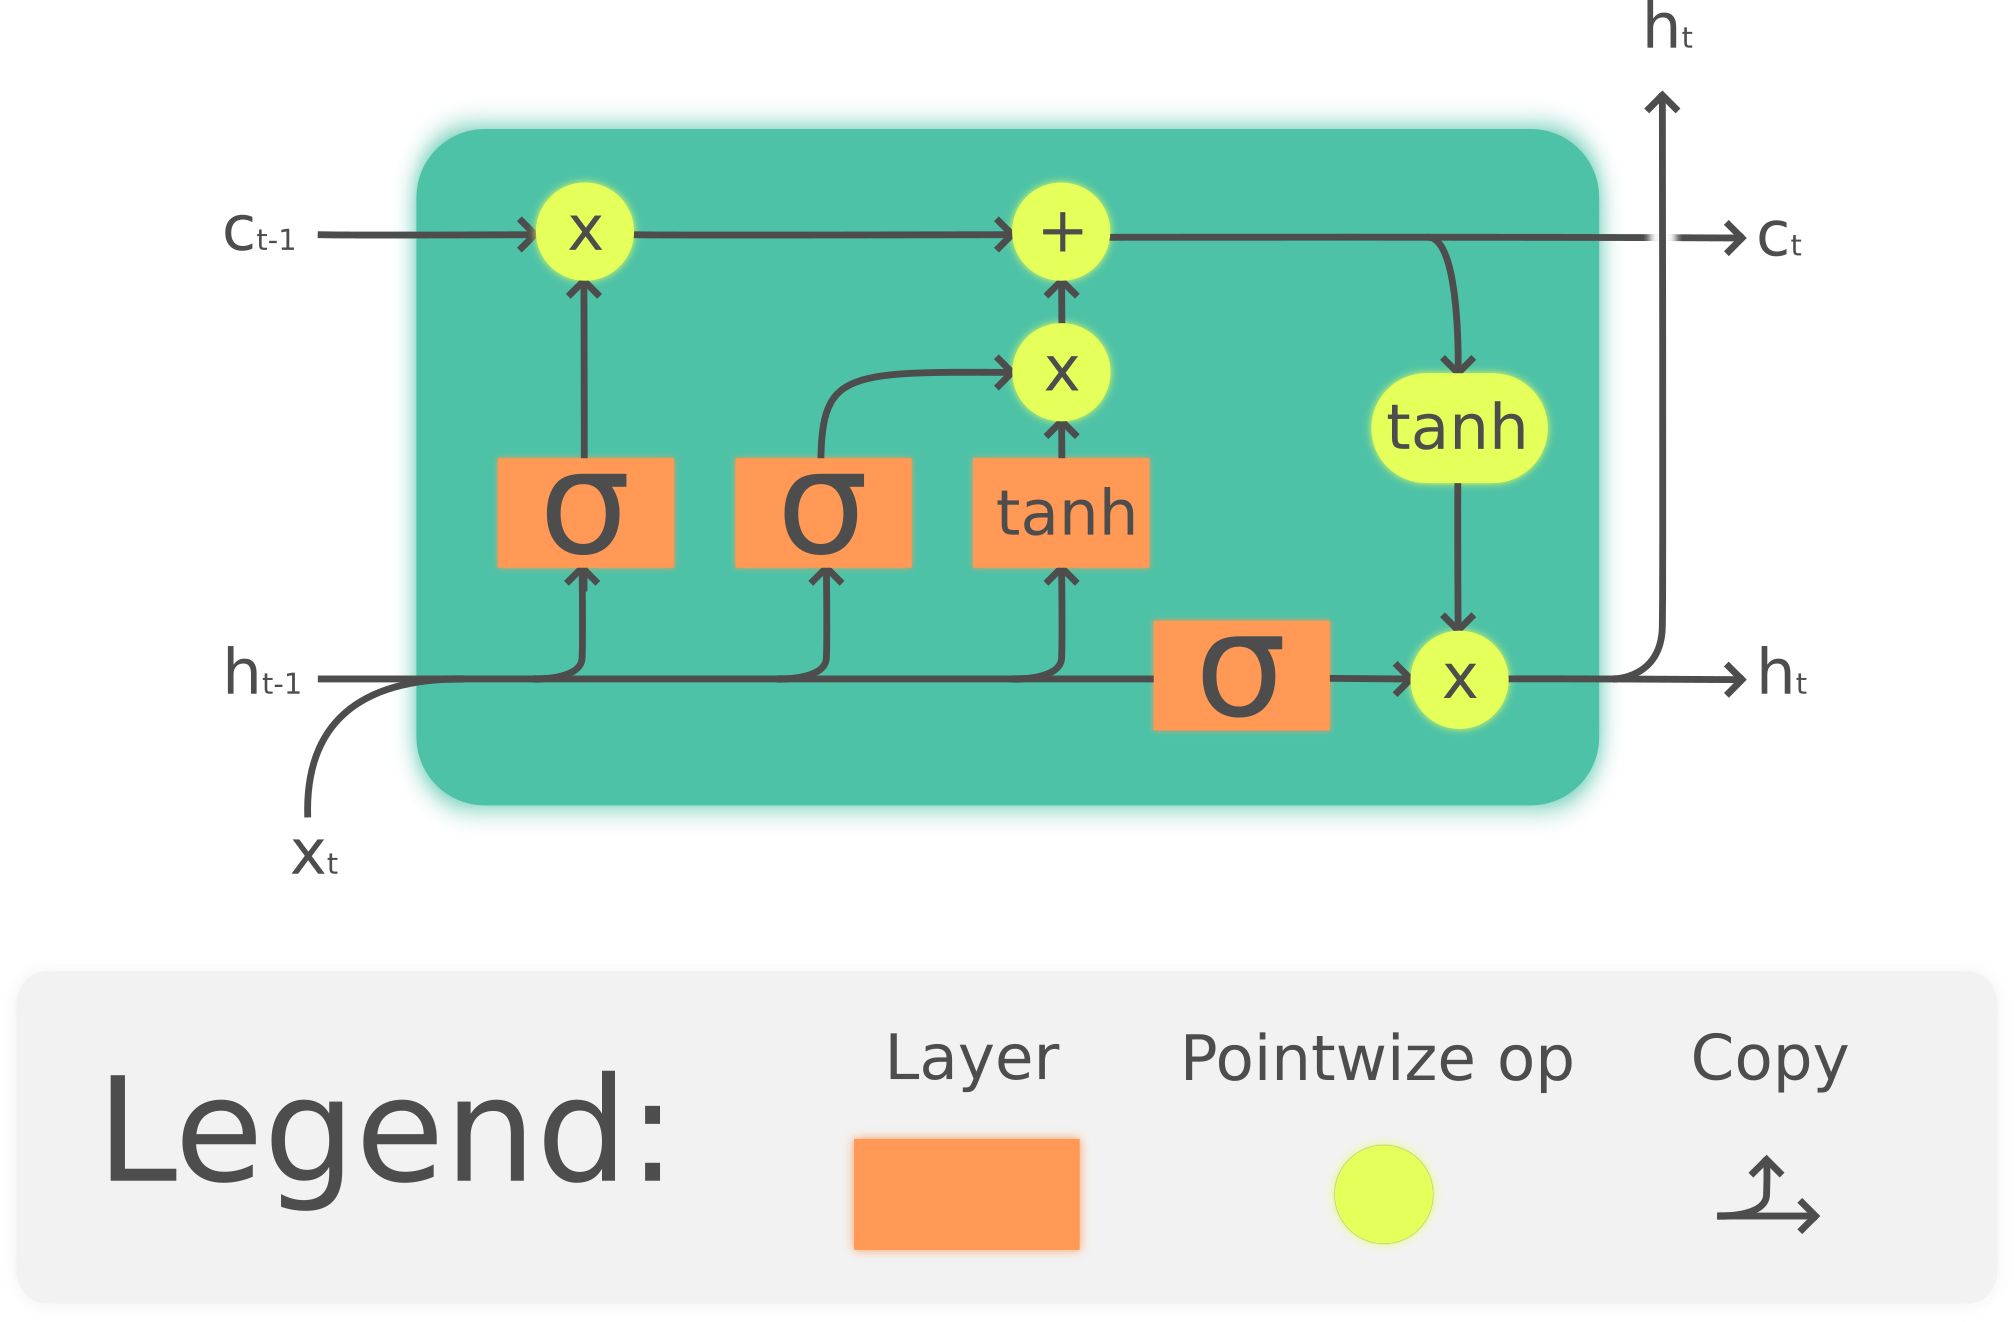
\includegraphics[width=\columnwidth]{img/computational_unit}
	\caption{The computational unit of a LSTM with input from dataset $ x(t) $, output $ h(t) $ and context function $ c(t) $. The input of the unit at time $ t $ is $ x(t)h(t-1)c(t-1) $ .}
	\label{fig:computational_unit}
\end{figure}


\begin{figure}[!h]
	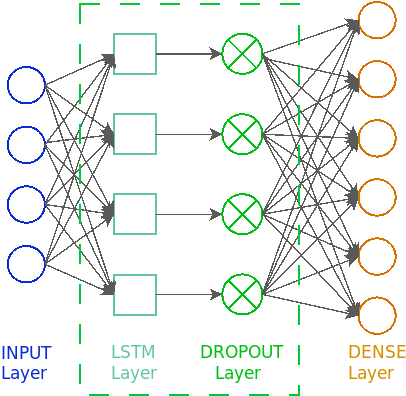
\includegraphics[width=\columnwidth]{img/LSTM}
	\caption{The general structure of the LSTM used in the experiment}
	\label{fig:LSTM}
\end{figure}
A LSTM neural network is made by at least one layer of LSTM units. The dataset to train a LSTM network in general is made by a sequence of input data and a corresponding sequence of output data.
In our specific case it has been created the structure of NN as in Figure \ref{fig:LSTM}.\\ 
In Table \ref{tab:params} there is the tuned hyperparameters values chosen for the experiment. Note that the total number of possible configuration of hyperparameters is $ 12*6*8*6 = 3456 $ however as will be shown, the number of trained model will be much less, decreasing the time to find good hyperparameters.\\
\begin{table}[!h]
	\caption{Table of the values to tune for the model. The chosen value for each parameter are: number of units per layer $ L_i $, Learning Rate ($ LR $), dropout percentage ($ D $) and number of LSTM layers ($ N $). }
	\begin{tabular}{ccccc}
		& $ L_i $ & $ LR $ 			& $ D $ & $ N $  \\ 
\hline
		1 & 25   & $ 10^{-1} $	& 0.05 & 1 \\
		2 & 50   & $ 10^{-2} $  & 0.10  & 2 \\
		3 & 75   & $ 10^{-3} $  & 0.15 & 3 \\
		4 & 100  & $ 10^{-4} $  & 0.20  & 4 \\
		5 & 125  & $ 10^{-5} $  & 0.25 & 5 \\
		6 & 150  & $ 10^{-6} $  & 0.30  & 6 \\
		7 & 175  &  			& 0.35 &   \\
		8 & 200  &  			& 0.40  &   \\
		9 & 225  &  			&      &   \\
		10 & 250 &  			&      &   \\
		11 & 275 &  			&      &   \\
		12 & 300 &  			&      &   \\
	\end{tabular}

\label{tab:params}
\end{table}

Let's now analyze the coding method to obtain the individual of the genetic algorithm from the LSTM trained model.


Nel nostro caso si propone di variare tra gli iperparametri il learning rate, la percentuale di Dropout e il numero di layer LSTM con il numero di unità sui rispettivi layer.
Fissiamo in tabella i valori dei parametri che vogliamo valutare e per collegarci all’algoritmo genetico definiamo l’individuo della popolazione come una n-upla formata dagli indici deii valori dei parametri corrispondenti. Supponendo di aver scelto un LR di 0.001, una percentuale di Dropout del 5 % e un singolo Layer LSTM con 4 unità computazionali, l’individuo corrispondente è rappresentato dalla seguente tupla.

\subsection{Genetic Algorithm}
Differenze da un comune GA:\\
• Paziente Zero\\
• Fitness calcolato da LSTM\\
• Non c’è un crossover\\
• Tutte le probabilità in gioco si basano sul modello di propagazione del Coronavirus\\

The following are the basics of this genetic algorithm.\\
\subsubsection{Individuals Population}
Super spreaders + infected / recovered / dead\\

\subsubsection{Populations}
The population divides individuals into 3 different (sub)populations, updated and maintained during the whole algorithm, in according with the type of individuals:
\begin{itemize}
\item Dead: It contains dead individuals. They can no longer be used in the algorithm.
\item Recovered: After each epoch, infected individuals are removed from their population and inserted here. These individuals can return to influence the algorithm if they are reinfected. Also individuals who simulate social distancing measures and therefore are isolated, belong to this population.
\item New-Infected: It holds all the new individuals that are infected in the previous epoch.
\end{itemize}

\subsubsection{Mutation}
• Numerous mutations\\
• Fixed part\\
• Variable part\\

\subsubsection{Propagation}
• Super spreaders => New infected and travel probability\\
• Population evolution every Iteration\\
\\
• Patient zero: fixed part + var part\\
while (epochs) {\\
propagateDisease ()\\
bestIndividualFound: infected / recovered / deaths\\
}\\
\\
1.propagateDisease () =\\
• Start from patient zero\\
• Step 1: Calculate each individual's fitness\\
• Step 2: sort the population by fitness\\
• Step 3: Save the best solution\\
• Step 4: idx super spreader and idx deaths\\
• Step 5: spreading the disease\\
o For each individual:\\
If idx> = idx deaths:\\
• kill him\\
If not:\\
• calculate the number of new ones infected by it:\\
• if idx <idx super spreader (is super spreader):\\
o ninfected = self.MIN SUPERSPREAD + random.randint (0, self.MAX SUPERSPREAD - self.MIN SUPERSPREAD)\\
• otherwise:\\
o ninfected = random.randint (0, self.MAX SPREAD)\\
• Calculate probability that the individual has "traveled": if he is a traveler:\\
or any individual can become infected (traverl distance = -1)\\
• if not: traverl distance = 1\\
• Cycle ninfected times:\\
o new infected = x.infect (travel distance = travel distance)\\
o If new infected does not belong to the list of deaths / infected / new infected list / recovered: Add it to the list new infected list\\
o If new infected belongs to recovered and does not belong to new infected list:\\
with prob. P REINFECTION add it to the new infected list list and remove it from recovered\\
• infected list is added to retrieved and the inferred list becomes the new infected\\
\\
2. individual.infected =\\
• copy the individual into a new one called mutated\\
• with ind probability, the individual can change his variable part\\
or change the 3rd value of the fixed part (= length var part) and then do the resizing of var part\\
or travel distance = -1\\
• if it changed: nmutated = random.randint (0, total size-1)\\
• if not: nmutated = 1\\
• cycle on nmutated:\\
or choose a random pos that is not the 3rd fixed part value and has not already been changed\\
o infectedPosition:\\
case 1: the fixed part-1 changes\\
case 2: change the varpart\\
=> choose max and min range and change from the old value to the previously calculated pos\\

\section{CVOA Meta-heuristic}

\section{Experiment Evaluation}

\section{Discussion of Differences}

\section{Conclusion}

\subsection{Future Work}

\printbibliography

\end{document}
